\section{Data center demand response}
\label{sec:DR_evaluation}

In this section, we extend the framework to study data center demand response (DCDR).


\subsection{Modeling data center demand response}
\begin{table}[!ht]
	\tbl{Demand response rates.\label{tbl:DR_rates}}{
	\begin{tabular}{|c|c|}
		\hline
		\textbf{Symbol}  &  \textbf{Value} (\$/kWh) \\ \hline \hline    
		
		$p_{tou}(t)$  & 0.05 (night), 0.219 (peak), 0.06 (off) \\     \hline
		$p^l_{ibr}$   & 0.2 ($l=1$: 50kW), 0.5 ($l=2$: 100kW), \\  \hline        
		$p_{cpp}$     & 11.2 \\ \hline
		$p_{sr}$      & 0.02  \\ \hline
		$p_{ws}$      & 0.05 \\ 
		\hline
	\end{tabular}}
\end{table}

To model DCDR, the proposed framework is modified for including the costs of participating in DR programs into the objective function a part of \textit{UtilBill}. In particular, we consider the following five DR programs:
\begin{itemize}
	\item Time-of-Use (ToU) rates, $p_{tou}(t)$, are defined based on the different times during a day, such as night time, peak time, and off-peak time \cite{ToURates}.
	\item Inclining block rates (IBR) encourage customers to consume electricity under some level, $l$, by charging a higher price, denoted by $p^l_{ibr}$, for the exceeding electricity usage.
	\item Under coincidence peak pricing (CPP) programs, industrial consumers like data centers are charged at a very high price, $p_{cpp}$, (e.g. than 200 times) for the usage during coincident peaks \cite{liu2013data}. For example, the CPP time is an hour per month selected by the utility company.
	\item In spinning reserve (SR) service, electricity customers are rewarded based on predefined SR rates if they reduce their load after receiving an SR signal command. 
	\item The rates $p_{ws}$ in wholesale markets are typically cheaper than the regular electricity prices. The participations of data centers in wholesale markets allow electricity suppliers to efficiently plan their generation.
\end{itemize}
The DR rates are summarized in Table \ref{tbl:DR_rates}.

\subsection{Numerical results}
\hideit{
\begin{figure*}[!ht]
	\begin{center} 
		\subfigure[Without DR programs. Data centers only use the grid power as the base prices of electricity are cheap. ]{{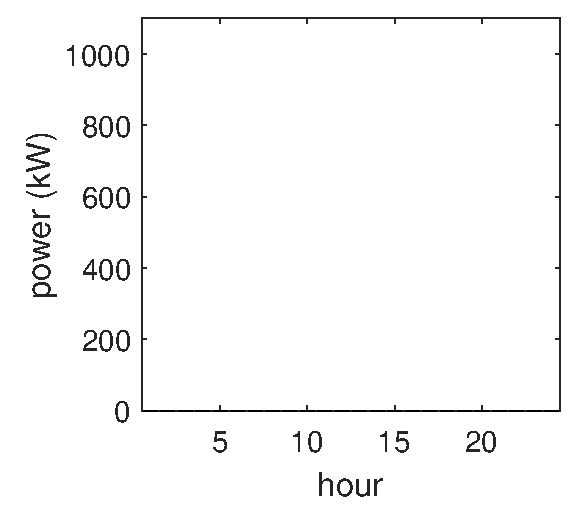
\includegraphics[width=0.32  \columnwidth]{figs/nz-int_NoDR}} 
			\label{fig:No_DR_program}    }
		\subfigure[Time of Use (ToU). Data centers provision 3 types of power sources during peak-hours.]{{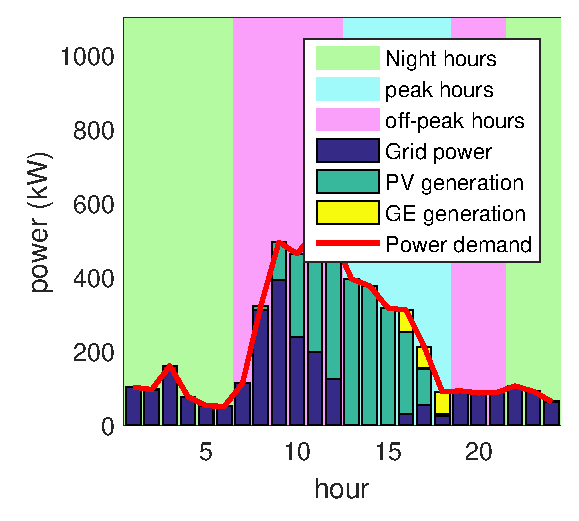
\includegraphics[width=0.32  \columnwidth]{figs/nz-int_tou}} 
			\label{fig:DR_programs_tou}   }
		\subfigure[CPP. Data centers prefer to use GE generation and PV generation in CPP hours.]{{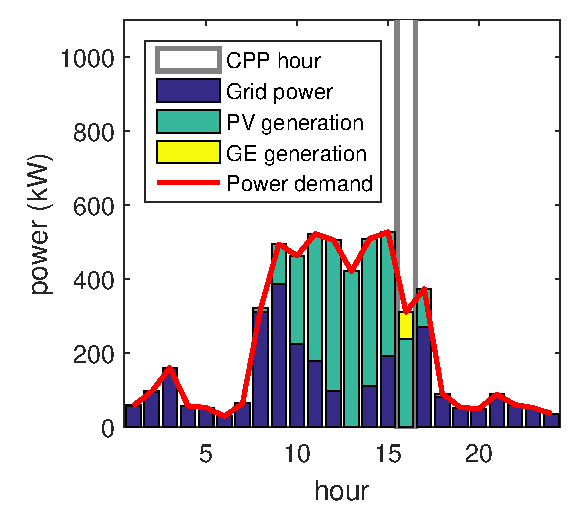
\includegraphics[width=0.32 \columnwidth]{figs/nz-int_cpp}} 
			\label{fig:DR_programs_cpp}    }
		\subfigure[IBR. The data center almost provisions its grid power under the IBR levels. ]{{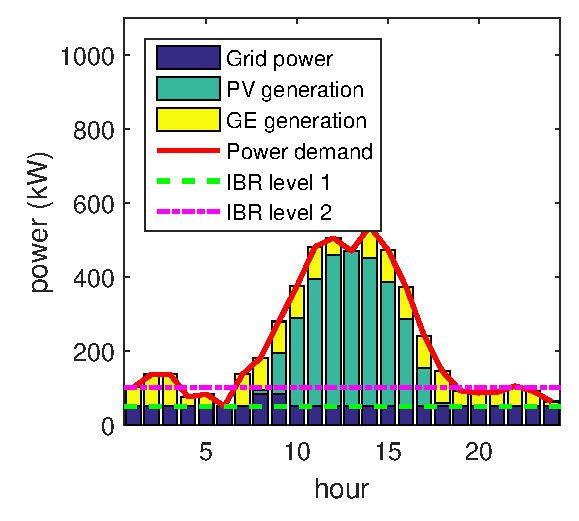
\includegraphics[width=0.32  \columnwidth]{figs/nz-int_ibr}} 
			\label{fig:DR_programs_ibr}    }
		\subfigure[Spinning reserve (SR). The data center reduces the grid power during SR hour to earn the SR reward. ]{{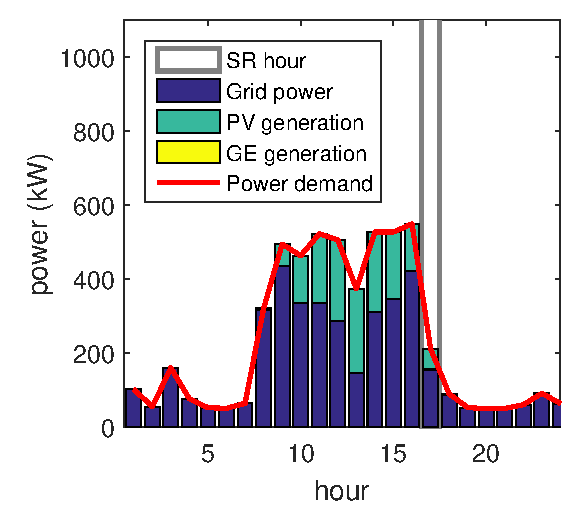
\includegraphics[width=0.32  \columnwidth]{figs/nz-int_sr}} 
			\label{fig:DR_programs_sr}    } 
		\subfigure[Wholesale (WS). The data center flattens the power demand to follow the pre-purchased power.]{{\includegraphics[width=0.32  \columnwidth]{figs/nz-int_BiMarkets}} 
			\label{fig:DR_programs_BiMarkets}    }        
		\caption{The power profiles of the data centers participating in different DR programs.}         
		\label{fig:DR_power_profiles}
	\end{center}
\end{figure*}

\begin{figure*}[!h]
	\begin{center}
		\subfigure[Capacity]{{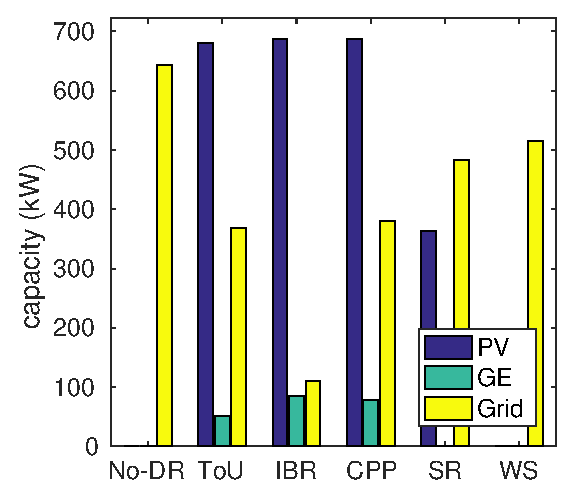
\includegraphics[width=0.32  \columnwidth]{figs/capacity_int_DR}} 
			\label{fig:DR_programs_capacity}    }
		\subfigure[Expenditures]{{\includegraphics[width=0.32  \columnwidth]{figs/cost_int_DR}} 
			\label{fig:DR_programs_cost}    }
		\subfigure[Emissions]{{\includegraphics[width=0.32  \columnwidth]{figs/emission_int_DR}} 
			\label{fig:DR_programs_emission}    }
		\caption{Impacts of DR programs on capacities, expenditures, and emissions of the data center. }         
		\label{fig:DR_programs}
	\end{center}
	\vspace{-0.5cm}
\end{figure*}
}
The numerical results are to study the impacts of DR programs on a data center using our proposed framework within a year. We answer the following two questions: How does the power profile of data center look like when participating in DR programs? How do DR programs impact on costs and emissions? 

Figure \ref{fig:DR_power_profiles} presents the typical daily power profiles of data centers participating in the DR programs. There are six cases: (1) Data centers do not participate in any DR programs, and data centers participate in (2) the ToU pricing program, (3) the CPP program, (4) the IBR program, (5) the SR ancillary service program, and (6) the wholesale market.

In the case of without any DR programs in Figure \ref{fig:No_DR_program}, the data center prefers to provision only the grid power because the electricity price is relatively cheaper than using GE and PV. In addition, the proposed framework does not need to schedule the batch jobs as the electricity price is fixed.

Figure \ref{fig:DR_programs_tou} illustrates the power profiles of the data center in the ToU program. We have 3 ToU price levels for off-peak hours $\$0.06/kWh$, night hours $\$0.05/kWh$, and peak hours $\$0.219/kWh$ \cite{Shahan2011ToUTexas}. The rates of night hours are the cheapest while the electricity rates of peak hours are the most expensive. The data center provisions PV and GE generation to reduce the electricity bill during peak hours. As the peak of PV generation is in the peak hours, PV generation contributes the most power during peak hours. Compared to Figure \ref{fig:No_DR_program}, the power demand is shifted to match the PV generation and avoid the high peaks during the peak hours. When the PV generation goes down within the ToU peak hours, the data center operates GE to serve the power demand. During off-peak hours, the data center prefers to use PV generation if available, then imports the energy from the electricity grid if necessary. Furthermore, the peak of power demand is not at the peak hours compared to the case of without any DR programs. However, why does the data center not shift the power demand from the off-peak hours (7 am - 12 pm) to the night hours (9 pm 6 am)? Because the interactive workload and batch jobs are colocated in the same servers, scheduling the batch jobs may increase the idle power.

Figure \ref{fig:DR_programs_cpp} shows the case of the data center participating in the CPP program. During the CPP hour, the data center needs to avoid using the grid power because the CPP rate is too high. Therefore, the data center provisions GE generation and utilizes PV generation during the CPP hour. A larger amount of PV generation is used compared to the case without DR programs. The power demand management schedules the batch job workload to react to the shape of PV generation, which has the peak in the afternoon.

We study the power profile of the data center with respect to two IBR levels which are level 1 (50kW) and level 2 (100kW) as in Figure \ref{fig:DR_programs_ibr}. The electricity prices of exceeding the level 2 grid power is $\$0.5$/kWh, more expensive than the level 1, i.e., $\$0.2$/kWh.  The idea of IBR is to regulate the power demand under the two load levels. As we expected, the data center adapts to the IBR program very well. In particular, the grid power is mostly under the level 1 and never exceeds the level 2. In order to provision power under the IBR levels, the data center actually requires a lot of PV generation and GE generation. The batch job workload is shifted to the high peak of PV generation during day time. On the other hand, GE is used in the whole day.

Figure \ref{fig:DR_programs_sr} presents the operation of the data center in the SR program. In the SR program, the data center can earn financial benefits if it reduces the power demand compared to the baseline consumption. In this simulation, the baseline consumption is the power consumption of the data center without participating in any DR program. We run the optimization framework to minimize the total cost for the data center in the DR program. During the SR hour, the data center reduces 30\% their grid power consumption as compared to the case without DR programs.

In the wholesale market, it is assumed that the data center provisions 200kWh every hour at a cheaper price (0.05 \$/kWh) than the base price (0.056 \$/kWh). The power profile of data center is in Figure \ref{fig:DR_programs_BiMarkets}. It is seen that the power demand is flattened to follow the pre-purchased electricity in the wholesale market. The data center significantly reduces its peak compared to the case without DR programs, which can be very beneficial to reduce the peak demand of the electricity grid.

The comparison of the six cases of data center demand response in terms of capacities, costs, and emissions are shown in Figures \ref{fig:DR_programs}. In general, the proposed framework enables the data center to adapt to each DR program very well. The data center increases the capacities of GE and/or PV under the ToU, CPP, IBR, and SR programs as in Figure \ref{fig:DR_programs_capacity}. Hence, the DR programs can indirectly change the capacity planning of data centers.
In Figure \ref{fig:DR_programs_cost}, the total costs of the data center increase in the ToU, IBR, and CPP programs but they decrease in the SR program and the wholesale market. The lowest expenditure is in the wholesale market because of the cheap electricity price but it releases the most emissions as the grid power is generated by mainly using the fossil fuel. Participating in ToU, IBR, and CPP programs causes the data center spends slightly more expenditures, but data centers can remarkably reduce emissions by using other environmentally friendly power sources rather than the grid power. 

\textbf{Key insights:} The proposed framework enables data centers to adapt to DR programs very well. (i) The data center uses a lot of PV and/or GE generation under ToU, IBR, CPP, and SR. (ii) While the total cost of the data center slightly increases in the ToU, CPP, and IBR programs, it can be reduced in the SR program and wholesale market. (iii) Data centers participating in ToU, IBR, CPP, and SR programs can cut down their emissions by provisioning other power sources rather than grid power.